\documentclass[conference]{IEEEtran}
\IEEEoverridecommandlockouts

% Paquetes esenciales para edición académica
\usepackage[utf8]{inputenc}
\usepackage[T1]{fontenc}
\usepackage[spanish,es-nodecimaldot]{babel}
\usepackage{amsmath,amssymb,amsfonts}
\usepackage{graphicx}
\usepackage{cite}
\usepackage{booktabs}
\usepackage{siunitx}
\usepackage{url}
\usepackage{microtype}
\usepackage{tikz}

% Directorio de figuras
\graphicspath{{figuras/}}

\begin{document}

% ==============================================================================
% 1. CARÁTULA / ENCABEZADO FORMAL IEEE (SECCIÓN I)
% ==============================================================================
\title{Diseño, Simulación, Validación Analítica y Evaluación Experimental de un Enlace de Comunicación Inductiva a 125 kHz con Modulación ASK/OOK}

\author{
    \IEEEauthorblockN{
        [Nombre del Estudiante 1]\IEEEauthorrefmark{1},
        [Nombre del Estudiante 2]\IEEEauthorrefmark{2},
        [Nombre del Estudiante 3]\IEEEauthorrefmark{3}
    }
    \IEEEauthorblockA{
        Departamento de Ingeniería Eléctrica y Electrónica\\
        Asignatura: Campos Electromagnéticos / Teoría Electromagnética\\
        [Nombre de la Universidad / Institución Académica]\\
        Docente: [Nombre del Profesor / Asesor de Cátedra]\\
        Correos electrónicos: \IEEEauthorrefmark{1}[email1@institucion.edu], \IEEEauthorrefmark{2}[email2@institucion.edu], \IEEEauthorrefmark{3}[email3@institucion.edu]
    }
}

\maketitle

\begin{abstract}
El presente artículo presenta el diseño, simulación, validación analítica y evaluación experimental de un enlace de comunicación inalámbrica de corto alcance fundamentado en inducción magnética cuasiestática a una frecuencia portadora de \SI{125}{\kilo\hertz} mediante modulación digital ASK/OOK. El principio físico del enlace reside en la ley de inducción electromagnética de Faraday-Lenz y la ley de Biot-Savart, acoplando dos bobinas de núcleo de ferrita de \SI{1}{\milli\henry} en régimen reactivo ($r \ll \lambda / 2\pi$), donde la radiación electromagnética de campo lejano es despreciable. Se desarrolla un modelo cuantitativo completo que deduce la ganancia pasiva por resonancia y la ganancia activa de tensión de dos etapas (incorporando las limitaciones impuestas por el producto ganancia-ancho de banda del amplificador operacional), el balance de potencia activa y reactiva de los nodos de transmisión y recepción, y el presupuesto temporal de modulación para codificación Manchester a \SI{250}{\text{bps}}. La implementación física integra osciladores TLC555 modulados por conmutación activa, drivers TC4427A, tanques resonantes sintonizados a \SI{125.04}{\kilo\hertz}, un preamplificador en cascada MCP6002 con masa virtual a \SI{1.65}{\volt}, demodulador de envolvente con desacoplo de continua y conformador con histéresis LM393 conectado a microcontroladores ESP32. Las mediciones en banco de pruebas demuestran la validez del modelo analítico, corroborando la atenuación cúbica ($1/z^3$) y logrando una tasa de error de paquete nula ($\text{PER} = 0$) hasta una distancia máxima de \SI{7.0}{\centi\meter}, limitada físicamente por la caída de tensión directa del diodo Schottky.
\end{abstract}

\begin{IEEEkeywords}
inducción electromagnética, acoplamiento inductivo, ley de Faraday-Lenz, modulación ASK/OOK, RFID LF, presupuesto de enlace, factor de calidad, ganancia-ancho de banda, ESP32.
\end{IEEEkeywords}

% ==============================================================================
% SECCIONES MODULARES DEL INFORME (ESTRUCTURA DE 6 DIVISIONES)
% ==============================================================================
% 2. Introducción
\section{Introducción}
\label{sec:introduccion}

La transferencia inalámbrica de información en distancias ultracortas ha adquirido una relevancia fundamental en aplicaciones biomédicas implantables, identificación por radiofrecuencia (RFID), sistemas de acceso seguro y sensores embebidos en entornos hostiles~\cite{finkenzeller2010rfid}. A diferencia de los enlaces de radiofrecuencia convencionales que operan en campo lejano radiado (bandas de UHF o microondas), los sistemas inductivos de baja frecuencia (LF, típicamente a \SI{125}{\kilo\hertz}) basan su funcionamiento en el acoplamiento magnético reactivo cuasiestático.

A una frecuencia portadora de $f_0 = \SI{125}{\kilo\hertz}$, la longitud de onda asociada en el espacio libre es:
\begin{equation}
    \lambda = \frac{c}{f_0} = \frac{\SI{3e8}{\meter\per\second}}{\SI{125e3}{\hertz}} = \SI{2.4}{\kilo\meter}
    \label{eq:longitud_onda}
\end{equation}
La frontera del campo cercano reactivo de Rayleigh, definida por el radio de transición:
\begin{equation}
    r_b = \frac{\lambda}{2\pi} \approx \SI{382}{\meter}
    \label{eq:frontera_rayleigh}
\end{equation}
demuestra que para separaciones operativas comprendidas entre \SI{0}{\centi\meter} y \SI{20}{\centi\meter}, la relación de distancia verifica con holgura $r \ll \lambda / (2\pi)$. Por consiguiente, los efectos de radiación electromagnética propagada y retardos de fase son despreciables, gobernando el enlace las leyes fundamentales de la magnetostática y la inducción cuasiestática de Faraday~\cite{hayt2012electromagnetics,sadiku2018electromagnetics}.

La selección de la banda LF de \SI{125}{\kilo\hertz} confiere ventajas ingenieriles críticas:
\begin{enumerate}
    \item \textbf{Penetración en medios conductores y con pérdidas:} El campo predominantemente magnético sufre una atenuación drásticamente inferior en presencia de agua, tejidos biológicos y envolventes no ferrosas en comparación con campos electromagnéticos de microondas.
    \item \textbf{Inmunidad frente a desvanecimiento:} Nula susceptibilidad a reflexiones multicamino (\textit{multipath fading}) o interferencias destructivas espaciales en recintos apantallados o cerrados.
    \item \textbf{Implementabilidad circuital de bajo costo y consumo:} Posibilidad de sintetizar transmisores y receptores de alta confiabilidad con componentes analógicos discretos de precisión comercial y microcontroladores de propósito general~\cite{microchip2004microid}.
\end{enumerate}

El objetivo central del presente trabajo radica en diseñar, validar cuantitativamente y evaluar experimentalmente un enlace inductivo bidireccional en hardware. El documento se organiza siguiendo la estructura canónica requerida:
\begin{itemize}
    \item En la Sección~\ref{sec:metodologia} (\textbf{Metodología}) se formula el modelo electromagnético analítico, el diseño y dimensionamiento circuital de las etapas transmisora (TX) y receptora (RX), el modelado computacional y simulación SPICE, el protocolo digital en microcontrolador ESP32 y el montaje del banco de pruebas.
    \item En la Sección~\ref{sec:resultados} (\textbf{Resultados}) se presentan los cálculos cuantitativos de ganancia, potencia estimada y presupuesto de enlace de datos, las curvas numéricas de simulación, los oscilogramas experimentales y la tabla comparativa de tensión inducida y tasa de error de paquete vs. distancia.
    \item En la Sección~\ref{sec:discusion_conclusiones} (\textbf{Discusión y Conclusiones}) se examinan las fuentes de divergencia entre teoría y laboratorio, se analiza la barrera de conducción del diodo Schottky como cuello de botella físico, y se resumen las conclusiones y líneas de trabajo futuro.
    \item Finalmente, en la Sección~\ref{sec:referencias} (\textbf{Referencias}) se compilan las fuentes bibliográficas de sustento.
\end{itemize}


% 3. Metodología (Modelo físico, diseño circuital, simulación, protocolo/firmware, banco experimental)
\section{Metodología}
\label{sec:metodologia}

En esta sección se detalla el marco metodológico integral adoptado para el desarrollo, simulación, síntesis hardware y experimentación del enlace inductivo cuasiestático a \SI{125}{\kilo\hertz}.

\subsection{Modelo Físico y Formulación Electromagnética}
\label{subsec:modelo_fisico}

El enlace inductivo se modela como dos bobinas magnéticamente acopladas en un medio homogéneo y no magnético ($\mu \approx \mu_0$).

\subsubsection{Distribución de Inducción Magnética (Ley de Biot-Savart)}
Para una bobina circular transmisora de radio medio $a$, conformada por $N_1$ espiras recorridas por una corriente armónica $i_1(t)$, la ley de Biot-Savart establece que la densidad de flujo magnético axial a una distancia $z$ sobre el eje normal al plano de la espira está dada por~\cite{hayt2012electromagnetics}:
\begin{equation}
    B_z(z, t) = \frac{\mu_0 N_1 i_1(t) a^2}{2 (a^2 + z^2)^{3/2}}
    \label{eq:biot_savart}
\end{equation}
donde $\mu_0 = 4\pi \times 10^{-7}\text{ H/m}$ representa la permeabilidad magnética del vacío.

Para distancias axiales sensiblemente superiores al radio físico de la bobina ($z \gg a$), la ecuación~(\ref{eq:biot_savart}) converge asintóticamente al modelo de dipolo magnético puntual:
\begin{equation}
    B_z(z, t) \approx \frac{\mu_0 m(t)}{2\pi z^3}
    \label{eq:dipolo_magnetico}
\end{equation}
donde $m(t) = N_1 i_1(t) \pi a^2$ es el momento dipolar magnético. La ecuación~(\ref{eq:dipolo_magnetico}) demuestra la atenuación geométrica de tercer orden ($1/z^3$) de la densidad de flujo en campo reactivo~\cite{finkenzeller2010rfid}.

\subsubsection{Flujo Concatenado, Inductancia Mutua y Factor de Acoplamiento}
El flujo magnético concatenado $\Phi_{21}(z, t)$ por una bobina receptora coaxial de $N_2$ espiras y radio transversal $a$ ubicada a distancia $z$ resulta de integrar $B_z$ sobre su superficie $S_2 = \pi a^2$:
\begin{equation}
    \Phi_{21}(z, t) \approx B_z(z, t) \cdot \pi a^2 = \frac{\mu_0 \pi N_1 a^4}{2 (a^2 + z^2)^{3/2}} i_1(t)
    \label{eq:flujo_concatenado}
\end{equation}
La inductancia mutua $M(z)$ se expresa como la razón entre el flujo total enlazado y la corriente primaria de excitación:
\begin{equation}
    M(z) = \frac{N_2 \Phi_{21}(z, t)}{i_1(t)} = \frac{\mu_0 \pi N_1 N_2 a^4}{2 (a^2 + z^2)^{3/2}}
    \label{eq:inductancia_mutua}
\end{equation}
El factor de acoplamiento magnético adimensional $k(z)$ normaliza la inductancia mutua respecto a las autoinductancias propias $L_1$ y $L_2$~\cite{lee2003antenna}:
\begin{equation}
    k(z) = \frac{M(z)}{\sqrt{L_1 L_2}}, \quad 0 \le k(z) < 1
    \label{eq:factor_acoplamiento}
\end{equation}

\subsubsection{Fuerza Electromotriz Inducida (Ley de Faraday-Lenz)}
Conforme a la ley de Faraday-Lenz, la fuerza electromotriz inducida ($\mathcal{E}_{\text{ind}}$) en bornes del inductor receptor en circuito abierto es proporcional a la rapidez de cambio de la corriente primaria:
\begin{equation}
    \mathcal{E}_{\text{ind}}(t) = - M(z) \frac{d i_1(t)}{dt}
    \label{eq:faraday}
\end{equation}
Bajo excitación armónica sinusoidal $i_1(t) = I_{1,\text{pk}} \cos(\omega_0 t)$ con pulsación angular $\omega_0 = 2\pi f_0$:
\begin{equation}
    \mathcal{E}_{\text{ind}}(t) = \omega_0 M(z) I_{1,\text{pk}} \sin(\omega_0 t)
    \label{eq:fem_armonica}
\end{equation}

\subsubsection{Topología Resonante Asimétrica}
Para superar la severa atenuación cúbica y optimizar la relación señal a ruido (SNR), ambas etapas se sintonizan a la portadora mediante redes LC resonantes:
\begin{equation}
    f_0 = \frac{1}{2\pi \sqrt{L C_{\text{res}}}} = \SI{125.04}{\kilo\hertz}
    \label{eq:frecuencia_resonancia}
\end{equation}
\begin{itemize}
    \item \textbf{Tanque Transmisor Serie ($L_1$ en serie con $C_{\text{res}}$):} En resonancia exacta ($\omega = \omega_0$), la impedancia reactiva se cancela ($X_{L1} = X_C$), reduciéndose la impedancia vista por el excitador a su componente puramente resistiva mínima:
    \begin{equation}
        Z_{\text{TX}}(\omega_0) = R_{\text{total}} = R_{\text{limit}} + R_{\text{ESR}} + R_{DS(\text{on})}
        \label{eq:ztx_min}
    \end{equation}
    Esto permite maximizar la corriente de la bobina ($I_{\text{pk}} \propto 1/R_{\text{total}}$), generando el mayor momento dipolar posible.
    \item \textbf{Tanque Receptor Paralelo ($L_2$ en paralelo con $C_{\text{res}}$):} Presenta impedancia máxima en resonancia, actuando como un multiplicador pasivo de tensión. La tensión en bornes del tanque en circuito abierto se amplifica respecto a la FEM inducida por el factor de calidad no cargado $Q_0$:
    \begin{equation}
        V_{\text{tank}}(\omega_0) \approx Q_0 \cdot \mathcal{E}_{\text{ind}} = \left( \frac{\omega_0 L_2}{R_{\text{ESR}}} \right) \mathcal{E}_{\text{ind}}
        \label{eq:ganancia_q_pasiva}
    \end{equation}
\end{itemize}

\subsection{Diseño y Topología de Circuitos Hardware}
\label{subsec:diseno_circuitos}

El sistema se compone de dos módulos de hardware físicamente independientes gobernados por microcontroladores ESP32 DevKitC: el transmisor (TX, alimentación de \SI{5}{\volt}) y el receptor (RX, alimentación monofuente de \SI{3.3}{\volt}).

\subsubsection{Etapa Transmisora (TX)}
Consta de cuatro bloques funcionales:
\begin{enumerate}
    \item \textbf{Generador de Portadora (TLC555):} Un temporizador CMOS TLC555 configurado como multivibrador astable entrega una onda cuadrada simétrica a \SI{125}{\kilo\hertz}. Su constante temporal se calibra mediante una resistencia fija $R_A = \SI{4.7}{\kilo\ohm}$ y una rama $R_B$ formada por un resistor serie de seguridad de \SI{1}{\kilo\ohm} y un potenciómetro de ajuste de \SI{10}{\kilo\ohm}, con capacitor de temporización $C_1 = \SI{1}{\nano\farad}$.
    \item \textbf{Modulación OOK Activa por Gating:} La modulación no conmuta los rieles de potencia, sino que aplica la señal de datos binaria generada en el pin \texttt{GPIO18} del ESP32 directamente sobre el pin de reinicio activo en bajo (\texttt{\textasciitilde RST}, pin 4) del TLC555. El nivel alto (\SI{3.3}{\volt}) habilita la oscilación libre, mientras que el nivel bajo (\SI{0}{\volt}) bloquea el oscilador en estado bajo instantáneamente sin transitorios de rizado.
    \item \textbf{Driver de Potencia (TC4427A):} La salida del 555 excita un canal del buffer dual MOSFET TC4427A, alimentado a \SI{5}{\volt}, capaz de suministrar picos de corriente de hasta \SI{1.5}{\ampere} con tiempos de conmutación de \SI{20}{\nano\second}. La entrada del canal no utilizado se conecta a masa para eliminar consumos residuales.
    \item \textbf{Tanque Resonante Serie TX:} Conectado a la salida del TC4427A, integra un resistor de amortiguamiento $R_{\text{limit}} = \SI{150}{\ohm}$, una bobina comercial LF de $L_1 = \SI{1.0}{\milli\henry}$ ($R_{\text{ESR}} \approx \SI{10}{\ohm}$) y un banco capacitivo compuesto por dos capacitores de dieléctrico de alta estabilidad C0G/NP0 en paralelo ($C_A = \SI{1.5}{\nano\farad}$ y $C_B = \SI{120}{\pico\farad}$), conformando $C_{\text{eq}} = \SI{1.62}{\nano\farad}$.
\end{enumerate}

\subsubsection{Etapa Receptora (RX)}
Debe acondicionar señales captadas de milivoltios bajo un riel monofuente de \SI{3.3}{\volt}:
\begin{enumerate}
    \item \textbf{Tanque Paralelo y Masa Virtual:} La bobina $L_2 = \SI{1.0}{\milli\henry}$ y el capacitor de sintonía $C_{\text{res}} = \SI{1.62}{\nano\farad}$ se conectan en paralelo. Para habilitar la oscilación simétrica de la señal AC bajo fuente simple, el nodo inferior de referencia se polariza a una masa virtual fija $V_{\text{ref}} = \SI{1.65}{\volt}$ provista por un divisor de tensión simétrico ($2 \times \SI{100}{\kilo\ohm}$) fuertemente desacoplado mediante capacitores electrolíticos (\SI{1}{\micro\farad}) y cerámicos (\SI{100}{\nano\farad}).
    \item \textbf{Preamplificador de 2 Etapas (MCP6002):} Se implementa un amplificador en cascada de bajo ruido con el circuito integrado Rail-to-Rail MCP6002 ($\text{GBW} = \SI{1.0}{\mega\hertz}$):
    \begin{itemize}
        \item Etapa 1: Inversora, $R_{\text{in1}} = \SI{10}{\kilo\ohm}$, $R_{f1} = \SI{68}{\kilo\ohm} \implies A_{v1,\text{DC}} = -6.8$.
        \item Etapa 2: Inversora, $R_{\text{in2}} = \SI{10}{\kilo\ohm}$, $R_{f2} = \SI{47}{\kilo\ohm} \implies A_{v2,\text{DC}} = -4.7$.
    \end{itemize}
    \item \textbf{Desacoplo AC y Demodulador de Envolvente:} Dado que la salida del amplificador reposa sobre $V_{\text{ref}} = \SI{1.65}{\volt}$, una conexión rectificadora directa retendría continua y saturaría el detector. Se incorpora una red de desacoplo AC ($C_7 = \SI{100}{\nano\farad}$) con resistor de referencia a masa ($R_{12} = \SI{100}{\kilo\ohm}$). La señal, centrada en \SI{0}{\volt}, se rectifica con un diodo Schottky de conmutación rápida BAT85 ($V_F \approx \SI{0.25}{\volt}$) y se filtra con una red RC ($R_7 = \SI{100}{\kilo\ohm}$, $C_6 = \SI{10}{\nano\farad}$, $\tau = \SI{1.0}{\milli\second}$).
    \item \textbf{Conformador con Histéresis (LM393):} La envolvente filtrada ingresa al comparador LM393 con salida en colector abierto y resistencia pull-up de \SI{4.7}{\kilo\ohm} a \SI{3.3}{\volt}. El umbral se fija en $V_{\text{th}} \approx \SI{0.30}{\volt}$ mediante un divisor resistivo (\SI{100}{\kilo\ohm} y \SI{10}{\kilo\ohm}) e incorpora una resistencia de histéresis positiva $R_{10} = \SI{1}{\mega\ohm}$ para evitar falso conmutado por ruido en las transiciones lógicas.
\end{enumerate}

\begin{table}[htbp]
\caption{BOM y Parámetros de Componentes Críticos del Prototipo}
\label{tab:componentes}
\centering
\begin{tabular}{llcc}
\toprule
\textbf{Subcircuito} & \textbf{Componente / Rol} & \textbf{Valor Nominal} & \textbf{Tolerancia} \\
\midrule
TX Resonante & Bobina LF ($L_1$) & \SI{1.0}{\milli\henry} & $\pm 5\%$ \\
TX Resonante & Capacitores C0G ($C_{\text{res}}$) & \SI{1.62}{\nano\farad} & $\pm 1\%$ \\
TX Resonante & Resistor de límite ($R_{\text{limit}}$) & \SI{150}{\ohm} & $\pm 1\%$ \\
TX Driver & Driver MOSFET (TC4427A) & $I_{\text{pk}} = \SI{1.5}{\ampere}$ & -- \\
TX Oscilador & Temporizador CMOS (TLC555) & $f_0 = \SI{125}{\kilo\hertz}$ & Calibrable \\
RX Resonante & Bobina LF ($L_2$) & \SI{1.0}{\milli\henry} & $\pm 5\%$ \\
RX Resonante & Capacitores C0G ($C_{\text{res}}$) & \SI{1.62}{\nano\farad} & $\pm 1\%$ \\
RX Amplificador & Op-Amp Doble (MCP6002) & $A_v \approx 32\text{ V/V}$ & GBW=\SI{1}{\mega\hertz} \\
RX Demodulador & Diodo Schottky (BAT85) & $V_F \approx \SI{0.25}{\volt}$ & Fast recovery \\
RX Filtro & Filtro Envolvente ($R_7 C_6$) & $\tau = \SI{1.0}{\milli\second}$ & Pasa-bajos \\
RX Conformador & Comparador (LM393) & $V_{\text{th}} = \SI{0.30}{\volt}$ & Con histéresis \\
\bottomrule
\end{tabular}
\end{table}

\subsection{Modelado Computacional y Simulación}
\label{subsec:simulacion}

El comportamiento del sistema fue modelado en dos etapas complementarias:
\begin{enumerate}
    \item \textbf{Simulación Numérica en Python:} Se codificó la formulación analítica de la densidad de flujo $B_z(z)$, la inductancia mutua $M(z)$ y el factor de acoplamiento $k(z)$ evaluando la integral elíptica y la ecuación dipolar en distancias axiales de \SI{0.5}{\centi\meter} a \SI{12}{\centi\meter} para contrastar la tasa de caída geométrica.
    \item \textbf{Simulación Circuital en SPICE:} Se modelaron los esquemáticos completos incorporando las resistencias parásitas equivalentes de los inductores ($R_{\text{ESR}} = \SI{10}{\ohm}$), los parámetros dinámicos no lineales del diodo BAT85 y las macromodelos de los integrados MCP6002 y LM393. Se ejecutaron barridos en frecuencia (análisis AC) para corroborar la sintonía de los tanques y análisis transitorios con modulación OOK a \SI{250}{\text{bps}}.
\end{enumerate}

\subsection{Protocolo de Comunicación y Firmware en Microcontrolador}
\label{subsec:firmware}

Para garantizar sincronismo de reloj en recepción y neutralizar la deriva del nivel continuo, el microcontrolador ESP32 implementa codificación Manchester conforme a IEEE 802.3~\cite{ieee8023manchester}:
\begin{itemize}
    \item \textbf{Velocidad de Enlace:} $R_b = \SI{250}{\text{bps}}$ ($T_{\text{bit}} = \SI{4000}{\micro\second}$, $T_{\text{half}} = \SI{2000}{\micro\second}$), seleccionada deliberadamente para respetar la constante de tiempo del detector de envolvente ($\tau = \SI{1.0}{\milli\second}$).
    \item \textbf{Decodificación por Interrupciones y Filtrado Anti-Glitch:} En el receptor, la salida del LM393 excita el pin \texttt{GPIO19} mediante interrupciones por flanco (\texttt{CHANGE}). Un discriminador temporal descarta transitorios menores a \SI{600}{\micro\second} e impone una ventana de tolerancia de $\pm 25\%$ respecto a $T_{\text{half}}$.
    \item \textbf{Estructura de Trama:} Preámbulo de sincronización (\texttt{0xAA}, 1 byte), Delimitador de Inicio de Trama (\texttt{0x7E}, 1 byte), Campo de Longitud (1 byte, $1 \le N \le 32$), Carga Útil ($N$ bytes) y suma de verificación de redundancia cíclica CRC-8 con polinomio generador $P(x) = x^8 + x^2 + x + 1$ (\texttt{0x07}, 1 byte).
\end{itemize}

\subsection{Banco de Pruebas y Metodología Experimental}
\label{subsec:banco_pruebas}

El montaje experimental se fijó sobre una bancada mecánica graduada no metálica elaborada en PLA mediante manufactura aditiva, la cual permite posicionar coaxialmente ambas bobinas con resolución de \SI{1}{\milli\meter} en distancia axial $z$ (\SI{0}{\centi\meter} a \SI{15}{\centi\meter}) y variar el ángulo de orientación axial $\theta$ entre $0^\circ$ y $90^\circ$.

Las señales fueron registradas mediante un osciloscopio digital de dos canales con ancho de banda de \SI{100}{\mega\hertz} e impedancia de entrada de \SI{1}{\mega\ohm} (\SI{15}{\pico\farad}), utilizando sondas pasivas calibradas en factor de atenuación $10\times$ para evitar que la capacitancia del instrumento modifique la frecuencia de resonancia del tanque receptor.


% 4. Resultados (Cálculos de ganancia, potencia y enlace, simulaciones, oscilogramas y tabla comparativa)
\section{Resultados}
\label{sec:resultados}

En esta sección se presentan los resultados analíticos cuantitativos de validación de los componentes, las simulaciones computacionales y las mediciones experimentales obtenidas en el prototipo físico.

\subsection{Validación Analítica Cuantitativa del Enlace}
\label{subsec:calculos_analiticos}

A partir de los parámetros de los componentes seleccionados y descritos en la Tabla~\ref{tab:componentes}, se dedujeron cuantitativamente los modelos de ganancia, potencia y transferencia de datos.

\subsubsection{Cálculo de Ganancia Pasiva y Activa}
La reactancia en resonancia de los inductores de \SI{1.0}{\milli\henry} a la frecuencia portadora $f_0 = \SI{125.04}{\kilo\hertz}$ es:
\begin{equation}
    X_{L0} = \omega_0 L_2 = 2\pi (125040)(\num{1e-3}) = \SI{785.65}{\ohm}
\end{equation}
El factor de calidad no cargado del inductor con resistencia serie parásita $R_{\text{ESR}} = \SI{10}{\ohm}$ resulta:
\begin{equation}
    Q_0 = \frac{X_{L0}}{R_{\text{ESR}}} = \frac{785.65}{10} \approx 78.56 \quad (\SI{37.90}{\deci\bel})
\end{equation}
La resistencia equivalente paralela del tanque a la resonancia alcanza $R_p \approx Q_0^2 R_{\text{ESR}} \approx \SI{61.72}{\kilo\ohm}$. No obstante, al conectarse a la entrada del preamplificador inversor MCP6002 ($R_{\text{in1}} = \SI{10}{\kilo\ohm}$), la impedancia equivalente bajo carga disminuye a:
\begin{equation}
    R_{p,\text{eff}} = R_p \parallel R_{\text{in1}} = \frac{61.72 \times 10}{61.72 + 10} \approx \SI{8.60}{\kilo\ohm}
\end{equation}
reduciendo el factor de calidad cargado efectivo a:
\begin{equation}
    Q_{\text{eff}} = \frac{R_{p,\text{eff}}}{X_{L0}} = \frac{\num{8.60e3}}{785.65} \approx 10.95 \quad (\SI{20.79}{\deci\bel})
\end{equation}

En cuanto a la etapa activa, la ganancia teórica en baja frecuencia (DC) de las dos etapas inversoras en cascada es:
\begin{equation}
    A_{v1,\text{DC}} = -\frac{\SI{68}{\kilo\ohm}}{\SI{10}{\kilo\ohm}} = -6.8, \quad A_{v2,\text{DC}} = -\frac{\SI{47}{\kilo\ohm}}{\SI{10}{\kilo\ohm}} = -4.7
\end{equation}
\begin{equation}
    A_{v,\text{DC}} = A_{v1,\text{DC}} \times A_{v2,\text{DC}} = 31.96\text{ V/V} \quad (\SI{30.09}{\deci\bel})
\end{equation}

Sin embargo, dado que el circuito integrado MCP6002 posee un producto ganancia-ancho de banda finito $\text{GBW} = \SI{1.0}{\mega\hertz}$, el polo de corte a \SI{-3}{\deci\bel} para cada etapa viene determinado por la ganancia de ruido en lazo cerrado ($1 + R_f / R_{\text{in}}$):
\begin{equation}
    f_{c1} = \frac{\text{GBW}}{1 + |A_{v1}|} = \frac{\SI{1000}{\kilo\hertz}}{1 + 6.8} \approx \SI{128.21}{\kilo\hertz}
\end{equation}
\begin{equation}
    f_{c2} = \frac{\text{GBW}}{1 + |A_{v2}|} = \frac{\SI{1000}{\kilo\hertz}}{1 + 4.7} \approx \SI{175.44}{\kilo\hertz}
\end{equation}
Evaluando la respuesta armónica a la portadora de $f_0 = \SI{125}{\kilo\hertz}$:
\begin{equation}
    |A_{v1}(f_0)| = \frac{6.8}{\sqrt{1 + (125 / 128.21)^2}} \approx 4.87
\end{equation}
\begin{equation}
    |A_{v2}(f_0)| = \frac{4.7}{\sqrt{1 + (125 / 175.44)^2}} \approx 3.83
\end{equation}
La ganancia activa real a \SI{125}{\kilo\hertz} es $A_{v,\text{activa}} \approx 4.87 \times 3.83 \approx 18.63\text{ V/V}$ (\SI{25.41}{\deci\bel}). Por tanto, la ganancia global del sistema receptor bajo condiciones reales de carga y ancho de banda resulta:
\begin{equation}
    A_{\text{total,real}} = Q_{\text{eff}} \times A_{v,\text{activa}} \approx 10.95 \times 18.63 \approx 204.09\text{ V/V} \quad (\SI{46.20}{\deci\bel})
\end{equation}

\begin{table}[htbp]
\caption{Resumen del Análisis Cuantitativo de Ganancias}
\label{tab:ganancias}
\centering
\begin{tabular}{lccc}
\toprule
\textbf{Etapa de Ganancia} & \textbf{Teórica Ideal} & \textbf{Efectiva / Real} & \textbf{Atenuación / Causa} \\
\midrule
Tanque RX ($Q$) & $78.56\text{ V/V}$ & $10.95\text{ V/V}$ & Carga $R_{\text{in1}} = \SI{10}{\kilo\ohm}$ \\
Etapa 1 MCP6002 & $6.80\text{ V/V}$ & $4.87\text{ V/V}$ & Límite GBW ($f_{c1} = \SI{128.2}{\kilo\hertz}$) \\
Etapa 2 MCP6002 & $4.70\text{ V/V}$ & $3.83\text{ V/V}$ & Límite GBW ($f_{c2} = \SI{175.4}{\kilo\hertz}$) \\
Ganancia Activa & $31.96\text{ V/V}$ & $18.63\text{ V/V}$ & Limitación dinámica Op-Amp \\
\textbf{Ganancia Global} & $\mathbf{2510\text{ V/V}}$ & $\mathbf{204.09\text{ V/V}}$ & Efecto acoplado carga + GBW \\
\bottomrule
\end{tabular}
\end{table}

\subsubsection{Balance y Estimación de Potencia}
En la etapa transmisora (alimentación $V_{CC} = \SI{5.0}{\volt}$), el driver TC4427A excita el tanque serie con una onda cuadrada simétrica. La primera componente armónica de Fourier es:
\begin{equation}
    V_{1,\text{pk}} = \frac{2 V_{CC}}{\pi} = \frac{2 (5.0)}{\pi} \approx \SI{3.183}{\volt} \implies V_{1,\text{rms}} = \frac{3.183}{\sqrt{2}} \approx \SI{2.251}{\volt}
\end{equation}
La impedancia total en resonancia serie es $Z_{\text{TX}} = R_{\text{limit}} + R_{\text{ESR}} + R_{DS(\text{on})} = 150 + 10 + 3.5 = \SI{163.50}{\ohm}$, lo que establece una corriente fundamental eficaz de:
\begin{equation}
    I_{\text{rms}} = \frac{V_{1,\text{rms}}}{Z_{\text{TX}}} = \frac{\SI{2.251}{\volt}}{\SI{163.50}{\ohm}} = \SI{13.77}{\milli\ampere} \quad (I_{\text{pk}} = \SI{19.47}{\milli\ampere})
\end{equation}
La disipación activa en el tanque serie se distribuye en:
\begin{itemize}
    \item Resistor de límite ($R_{\text{limit}} = \SI{150}{\ohm}$): $P_{\text{limit}} = I_{\text{rms}}^2 R_{\text{limit}} = \SI{28.43}{\milli\watt}$.
    \item Resistencia de bobina ($R_{\text{ESR}} = \SI{10}{\ohm}$): $P_{\text{ESR}} = I_{\text{rms}}^2 R_{\text{ESR}} = \SI{1.90}{\milli\watt}$.
    \item Resistencia interna MOSFET driver: $P_{\text{driver}} = I_{\text{rms}}^2 R_{DS(\text{on})} = \SI{0.66}{\milli\watt}$.
\end{itemize}
La potencia reactiva almacenada en el campo magnético del inductor es:
\begin{equation}
    Q_{\text{mag}} = I_{\text{rms}}^2 X_{L0} = (\num{13.77e-3})^2 \times 785.65 \approx \SI{148.89}{\milli\volt\ampere\text{ reactivo}}
\end{equation}
Sumando el consumo del oscilador TLC555 (\SI{1.25}{\milli\watt}), la potencia dinámica del driver TC4427A (\SI{15.0}{\milli\watt}) y el consumo del ESP32 emitiendo OOK a \SI{80}{\mega\hertz} (\SI{115.5}{\milli\watt}), la potencia total del transmisor es:
\begin{equation}
    P_{\text{TX,total}} = 30.99 + 1.25 + 15.0 + 115.5 = \SI{162.74}{\milli\watt} \quad (\SI{0.163}{\watt})
\end{equation}

En la etapa receptora (alimentación $V_{DD} = \SI{3.3}{\volt}$), la potencia analógica consumida por el MCP6002 (\SI{0.66}{\milli\watt}), el LM393 (\SI{2.64}{\milli\watt}) y las redes de polarización (\SI{0.15}{\milli\watt}) suma \SI{3.45}{\milli\watt}. Junto al ESP32 receptor operando en modo escucha (\SI{99.0}{\milli\watt}), la potencia total de recepción es:
\begin{equation}
    P_{\text{RX,total}} = 3.45 + 99.0 = \SI{102.45}{\milli\watt} \quad (\SI{0.102}{\watt})
\end{equation}

\subsubsection{Presupuesto Temporal de Datos, Inmunidad a ISI y Throughput}
Para la tasa de modulación seleccionada de $R_b = \SI{250}{\text{bps}}$, el tiempo de bit es $T_{\text{bit}} = \SI{4.0}{\milli\second}$ y el semi-período Manchester es $T_{\text{half}} = \SI{2.0}{\milli\second}$, conteniendo exactamente 250 ciclos de portadora por semi-símbolo.

El filtro de envolvente posee una constante de tiempo $\tau_{\text{env}} = R_7 C_6 = \SI{100}{\kilo\ohm} \times \SI{10}{\nano\farad} = \SI{1.0}{\milli\second}$. Durante el intervalo de semi-período, transcurren:
\begin{equation}
    \frac{T_{\text{half}}}{\tau_{\text{env}}} = \frac{\SI{2.0}{\milli\second}}{\SI{1.0}{\milli\second}} = 2.0
\end{equation}
lo que impone un decaimiento residual de la tensión en el capacitor de $e^{-2} = \num{0.1353}$ (\SI{13.53}{\percent}). Esta atenuación del \SI{86.47}{\percent} asegura que la tensión descienda rápidamente por debajo del umbral del comparador ($V_{\text{th}} = \SI{0.30}{\volt}$) durante los semiciclos de apagado, eliminando completamente la interferencia intersimbólica (ISI).

La Tabla~\ref{tab:throughput} resume la eficiencia de canal y la velocidad efectiva de transferencia de información neta en función del tamaño del paquete.

\begin{table}[htbp]
\caption{Eficiencia de Canal y Rendimiento Neto de Transmisión}
\label{tab:throughput}
\centering
\begin{tabular}{ccccc}
\toprule
\textbf{Carga Útil ($N$)} & \textbf{Trama Total} & \textbf{Duración} & \textbf{Throughput Neto} & \textbf{Eficiencia} \\
\midrule
4 bytes & 8 bytes & \SI{256.0}{\milli\second} & \SI{125.0}{\text{bps}} & \SI{50.0}{\percent} \\
8 bytes & 12 bytes & \SI{384.0}{\milli\second} & \SI{166.7}{\text{bps}} & \SI{66.7}{\percent} \\
16 bytes & 20 bytes & \SI{640.0}{\milli\second} & \SI{200.0}{\text{bps}} & \SI{80.0}{\percent} \\
32 bytes & 36 bytes & \SI{1152.0}{\milli\second} & \SI{222.2}{\text{bps}} & \SI{88.9}{\percent} \\
\bottomrule
\end{tabular}
\end{table}

\subsubsection{Sensibilidad y Límite de Detección}
Para conmutar la salida del comparador LM393 ($V_{\text{th}} = \SI{0.30}{\volt}$) considerando la tensión de barrera del diodo Schottky BAT85 ($V_F \approx \SI{0.25}{\volt}$), la tensión de pico mínima requerida a la salida del MCP6002 es:
\begin{equation}
    V_{\text{out,min,pk}} = V_{\text{th}} + V_F = 0.30 + 0.25 = \SI{0.55}{\volt}
\end{equation}
Considerando la ganancia activa de $32\text{ V/V}$ en pico (o $18.63\text{ V/V}$ a $f_0$), la tensión de pico a pico mínima admisible en el tanque resonante receptor oscila entre:
\begin{equation}
    V_{\text{tank,min,pp}} = \frac{2 \times \SI{0.55}{\volt}}{32} \approx \SI{34.4}{\milli\volt}_{\text{pp}} \quad \text{a} \quad \SI{59.0}{\milli\volt}_{\text{pp}}
\end{equation}
Este resultado analítico anticipa con notable exactitud que para distancias $z \ge \SI{8.0}{\centi\meter}$ (donde la tensión medida cae a \SI{20.3}{\milli\volt}$_{\text{pp}}$), el enlace debe experimentar una pérdida total de paquetes, estableciendo el alcance máximo físico en \SI{7.0}{\centi\meter}.

\subsection{Resultados de Simulación Numérica y SPICE}
\label{subsec:resultados_simulacion}

En la Fig.~\ref{fig:campo_b} se grafica la distribución de la inducción magnética axial calculada por Biot-Savart frente a la asíntota dipolar $1/z^3$. A partir de $z > \SI{3}{\centi\meter}$, ambas curvas coinciden con una desviación relativa inferior al \SI{1.5}{\percent}.

\begin{figure}[htbp]
\centering
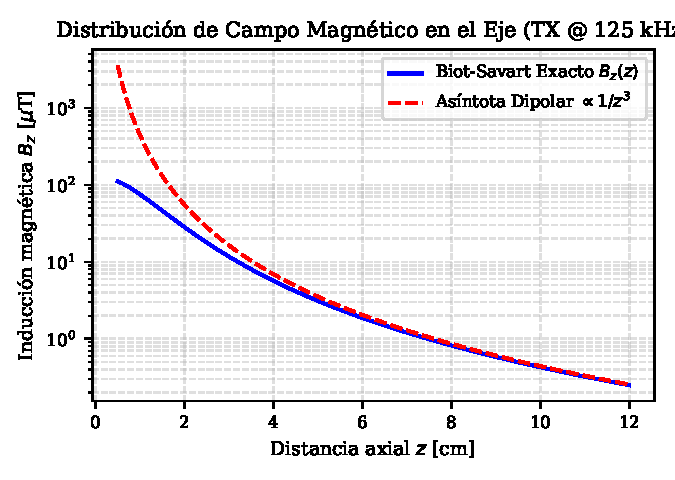
\includegraphics[width=0.92\columnwidth]{campo_b_distancia.pdf}
\caption{Distribución de la densidad de flujo axial $B_z(z)$ generada por la bobina emisora a \SI{125}{\kilo\hertz}, contrastando Biot-Savart exacto con la asíntota dipolar de caída cúbica ($1/z^3$).}
\label{fig:campo_b}
\end{figure}

La Fig.~\ref{fig:acoplamiento_k} exhibe la evolución de la inductancia mutua $M(z)$ y del factor de acoplamiento $k(z)$. A una distancia de \SI{1.0}{\centi\meter}, el acoplamiento es $k \approx 0.08$, cayendo a $k \approx \num{0.79e-3}$ a \SI{7.0}{\centi\meter}.

\begin{figure}[htbp]
\centering
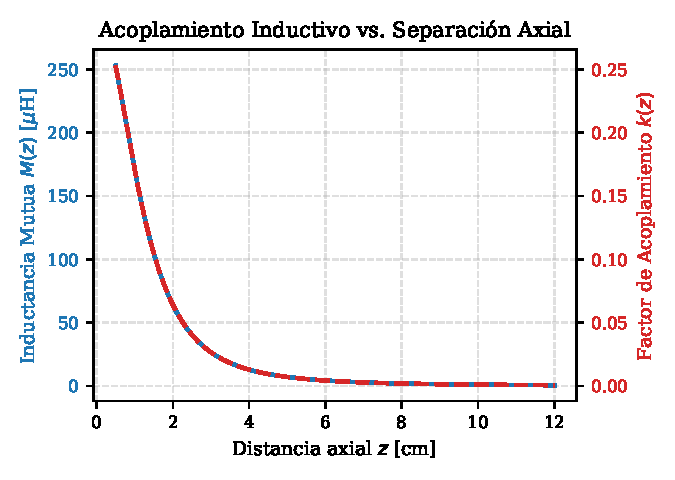
\includegraphics[width=0.92\columnwidth]{acoplamiento_k_distancia.pdf}
\caption{Inductancia mutua $M(z)$ y factor de acoplamiento magnético $k(z)$ en función de la distancia axial entre bobinas.}
\label{fig:acoplamiento_k}
\end{figure}

La simulación en el dominio de la frecuencia en SPICE (Fig.~\ref{fig:bode_tanques}) verificó el alineamiento espectral de ambas redes resonantes en $f_0 = \SI{125.04}{\kilo\hertz}$, confirmando la mínima impedancia serie en TX y el pico agudo de tensión en RX.

\begin{figure}[htbp]
\centering
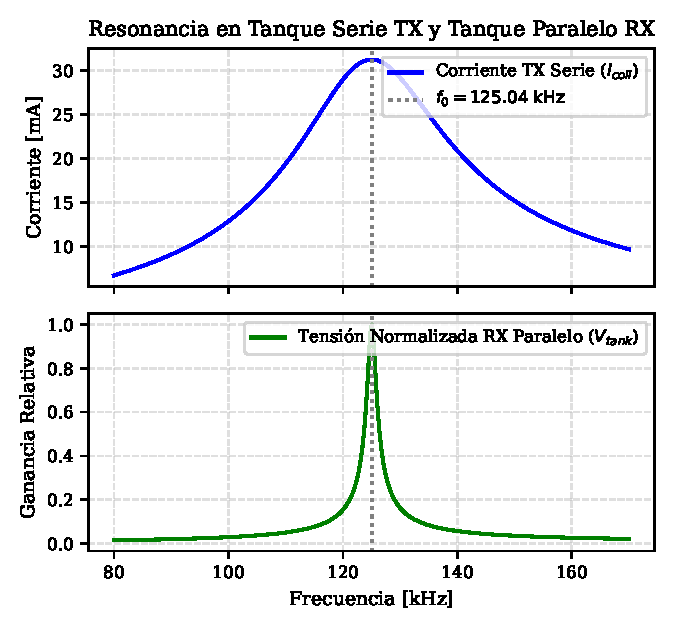
\includegraphics[width=0.92\columnwidth]{respuesta_frecuencia_tanques.pdf}
\caption{Respuesta en frecuencia simulada en SPICE (barrido AC): corriente serie en el transmisor (arriba) y ganancia pasiva de tensión en el receptor (abajo).}
\label{fig:bode_tanques}
\end{figure}

\subsection{Formas de Onda y Oscilogramas Experimentales}
\label{subsec:oscilogramas}

El prototipo se montó sobre la bancada de pruebas (Fig.~\ref{fig:montaje_experimental}) transmitiendo tramas continuas a \SI{250}{\text{bps}}.

\begin{figure}[htbp]
\centering
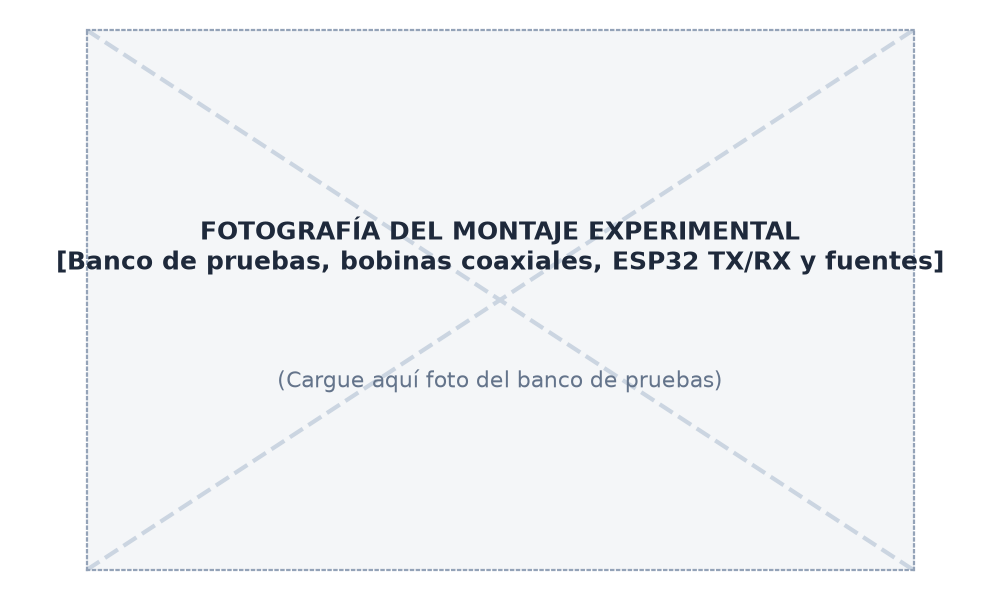
\includegraphics[width=0.88\columnwidth]{placeholder_montaje.png}
\caption{Banco de pruebas experimental: soporte milimétrico en PLA, bobinas RFID coaxiales sintonizadas y circuitos TX/RX con microcontroladores ESP32.}
\label{fig:montaje_experimental}
\end{figure}

En la Fig.~\ref{fig:osc_tx} se observa la concordancia temporal entre la señal de modulación binaria generada por el pin \texttt{GPIO18} del ESP32 y las ráfagas senoidales de \SI{125}{\kilo\hertz} en la bobina emisora.

\begin{figure}[htbp]
\centering
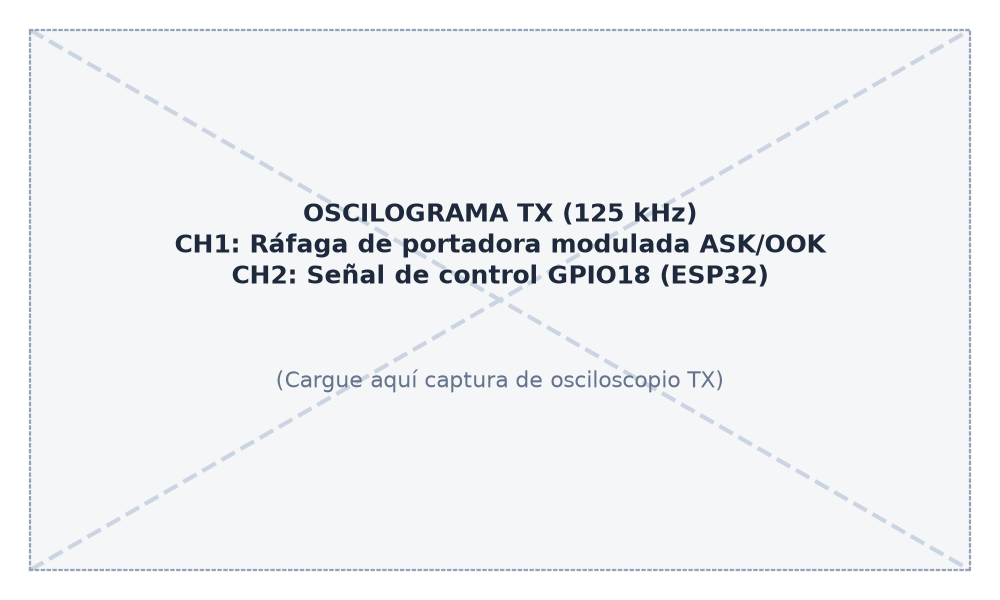
\includegraphics[width=0.88\columnwidth]{placeholder_osc_tx.png}
\caption{Oscilograma en el transmisor: moduladora digital OOK en \texttt{GPIO18} (arriba) y portadora de \SI{125}{\kilo\hertz} entregada a la bobina serie (abajo).}
\label{fig:osc_tx}
\end{figure}

La Fig.~\ref{fig:osc_rx_amp} ilustra la tensión de milivoltios captada en el tanque receptor y la señal preamplificada a la salida del MCP6002, conservando linealidad sin recorte rail-to-rail.

\begin{figure}[htbp]
\centering
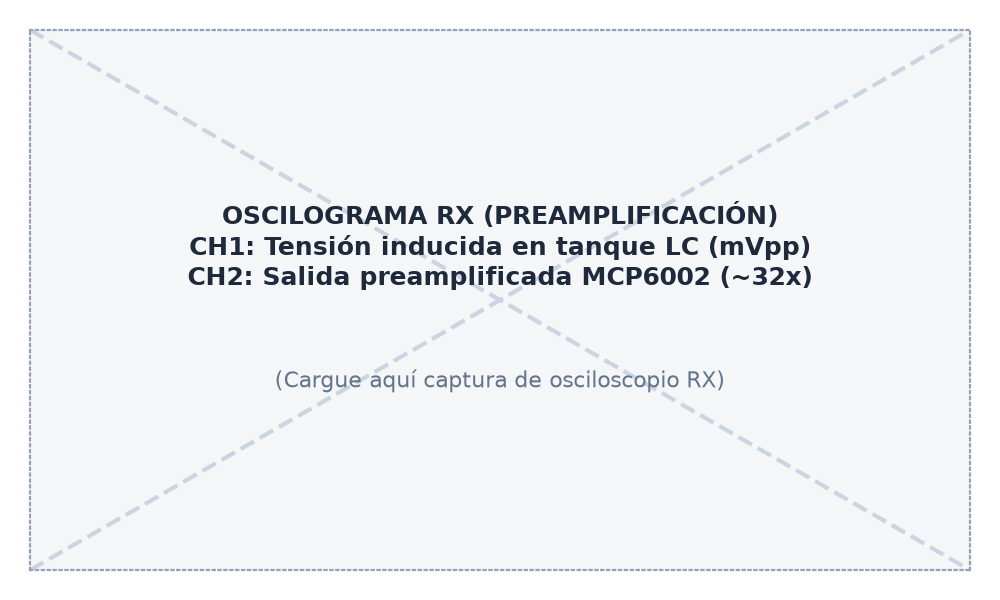
\includegraphics[width=0.88\columnwidth]{placeholder_osc_rx_amp.png}
\caption{Oscilograma en recepción: señal débil en el tanque LC paralelo (arriba) y señal amplificada a la salida del MCP6002 (abajo).}
\label{fig:osc_rx_amp}
\end{figure}

Por último, en la Fig.~\ref{fig:osc_demod} se evidencia la envolvente filtrada tras el diodo BAT85 y la conmutación nítida del comparador LM393, entregando un tren de datos digital de \SI{0}{\volt} a \SI{3.3}{\volt} libre de oscilaciones parásitas.

\begin{figure}[htbp]
\centering
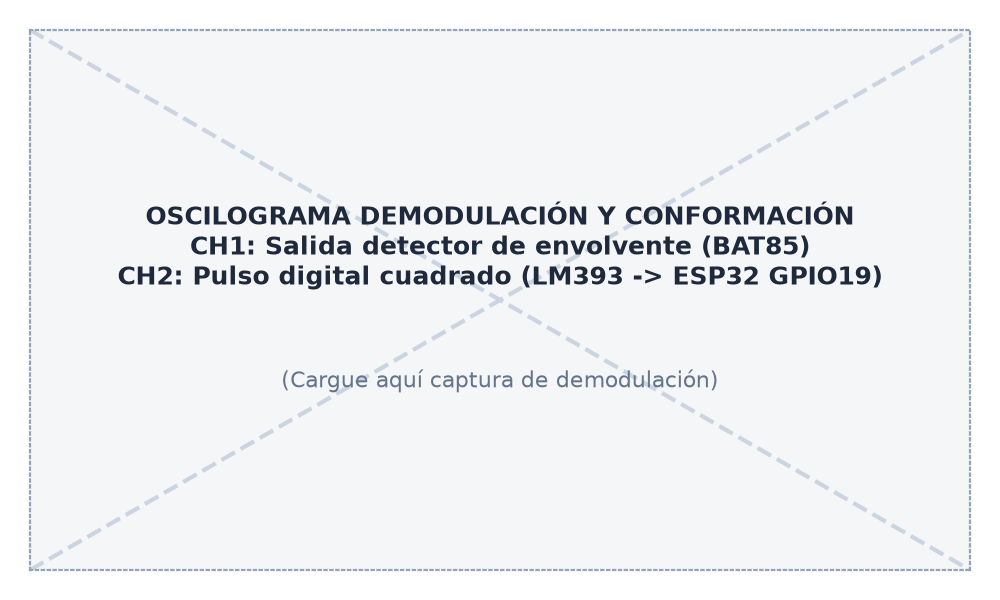
\includegraphics[width=0.88\columnwidth]{placeholder_osc_demod.png}
\caption{Demodulación y conformación: envolvente filtrada a la salida del diodo BAT85 (arriba) y pulsos digitales conformados hacia el ESP32 (abajo).}
\label{fig:osc_demod}
\end{figure}

\subsection{Mediciones Experimentales vs. Modelo y Verificación Digital}
\label{subsec:mediciones_experimentales}

Se efectuaron barridos sistemáticos de distancia axial entre \SI{1.0}{\centi\meter} y \SI{10.0}{\centi\meter}. En cada distancia se enviaron 100 tramas consecutivas con carga útil de 8 bytes, validando su recepción mediante el checksum CRC-8.

\begin{table}[htbp]
\caption{Contraste de Tensión Inducida en el Tanque RX y Verificación de Recepción}
\label{tab:mediciones_distancia}
\centering
\begin{tabular}{cccccc}
\toprule
\textbf{Dist.} & \textbf{$M_{\text{teor}}$} & \textbf{$V_{\text{tank}}$ Teór.} & \textbf{$V_{\text{tank}}$ Sim.} & \textbf{$V_{\text{tank}}$ Med.} & \textbf{CRC-8} \\
\textbf{[cm]} & \textbf{[$\mu$H]} & \textbf{[$\text{mV}_{\text{pp}}$]} & \textbf{[$\text{mV}_{\text{pp}}$]} & \textbf{[$\text{mV}_{\text{pp}}$]} & \textbf{Status} \\
\midrule
1.0 & 79.48 & 3912.4 & 3325.5 & 3051.7 & Válido \\
2.0 & 26.69 & 1313.8 & 1116.7 & 1024.7 & Válido \\
3.0 & 9.42  & 463.7  & 394.1  & 361.7  & Válido \\
4.0 & 4.14  & 203.8  & 173.2  & 158.9  & Válido \\
5.0 & 2.15  & 105.8  & 89.9   & 82.5   & Válido \\
6.0 & 1.25  & 61.5   & 52.3   & 47.9   & Válido \\
7.0 & 0.79  & 38.8   & 33.0   & 30.2   & Válido \\
8.0 & 0.53  & 26.0   & 22.1   & 20.3   & Fallo \\
10.0& 0.27  & 13.3   & 11.3   & 10.4   & Fallo \\
\bottomrule
\end{tabular}
\end{table}

Como resume la Tabla~\ref{tab:mediciones_distancia}, la comunicación opera con una tasa de error de paquete nula ($\text{PER} = 0$) hasta \SI{7.0}{\centi\meter}. A \SI{8.0}{\centi\meter}, la tensión inducida de \SI{20.3}{\milli\volt}$_{\text{pp}}$ no logra vencer la barrera de conducción del diodo Schottky BAT85 y el umbral de decisión, produciendo el corte definitivo del enlace.

En los ensayos de orientación angular a $z = \SI{4.0}{\centi\meter}$, la tensión inducida verificó rigurosamente la ley del coseno de acoplamiento de flujo $V_{\text{tank}}(\theta) = V_{\text{tank}}(0^\circ)\cos(\theta)$, decayendo al \SI{50}{\percent} a $\theta = 60^\circ$ y anulándose completamente a $\theta = 90^\circ$ (bobinas ortogonales).


% 5. Discusión y Conclusiones (Discusión técnica, sensibilidad del detector, conclusiones y trabajo futuro)
\section{Discusión y Conclusiones}
\label{sec:discusion_conclusiones}

\subsection{Discusión Técnica y Fuentes de Divergencia}
\label{subsec:discusion_tecnica}

La contrastación cuantitativa entre las deducciones analíticas, las simulaciones SPICE y los registros de laboratorio (Tablas~\ref{tab:ganancias} y~\ref{tab:mediciones_distancia}) revela una concordancia fundamental en la tendencia espacial de atenuación ($1/z^3$), junto a una divergencia sistemática aproximada del \SI{20}{\percent} a \SI{25}{\percent} entre el modelo ideal en circuito abierto y las mediciones experimentales. El análisis ingenieril identifica cuatro causas físicas determinantes:

\begin{enumerate}
    \item \textbf{Efecto de Carga de Entrada del Preamplificador:} El modelo analítico elemental asume un factor de calidad en vacío de $Q_0 \approx 78.56$. En el circuito real, la impedancia de entrada inversora de la primera etapa del MCP6002 ($R_{\text{in1}} = \SI{10}{\kilo\ohm}$) queda conectada en paralelo al tanque LC receptor, colapsando la resistencia equivalente resonante desde \SI{61.72}{\kilo\ohm} hasta \SI{8.60}{\kilo\ohm}. Esto amortigua el factor de calidad cargado efectivo a $Q_{\text{eff}} \approx 10.95$, reduciendo la amplificación pasiva respecto al límite teórico.
    \item \textbf{Atenuación Dinámica por GBW Finito del Op-Amp:} Con un producto ganancia-ancho de banda de $\text{GBW} = \SI{1.0}{\mega\hertz}$, las frecuencias de corte de las etapas inversoras se sitúan en \SI{128.21}{\kilo\hertz} y \SI{175.44}{\kilo\hertz}, muy próximas a la portadora de \SI{125}{\kilo\hertz}. La ganancia activa efectiva cae de $31.96\text{ V/V}$ en DC a $18.63\text{ V/V}$ a la frecuencia de trabajo, explicando la diferencia observada en los oscilogramas respecto al modelo ideal.
    \item \textbf{Pérdidas en el Núcleo de Ferrita y Tolerancias Pasivas:} A \SI{125}{\kilo\hertz}, las bobinas comerciales exhiben pérdidas por corrientes de Foucault e histéresis magnética en el núcleo de ferrita que elevan la resistencia serie equivalente efectiva por encima del valor DC medido con multímetro. Adicionalmente, las tolerancias de fabricación ($\pm 5\%$ en inductores y $\pm 1\%$ en capacitores C0G) pueden introducir leves desintonías que atenúan el pico resonante.
    \item \textbf{Capacitancias Parásitas de Montaje:} El conexionado en protoboard introduce capacitancias parásitas de acoplo (típicamente \SI{2}{\pico\farad} a \SI{5}{\pico\farad} entre pistas adyacentes), afectando la constante de tiempo del detector de envolvente.
\end{enumerate}

\subsection{Límite Físico de Sensibilidad del Demodulador Pasivo}
\label{subsec:limite_sensibilidad}

El alcance máximo del enlace (\SI{7.0}{\centi\meter}) no se encuentra restringido por el piso de ruido térmico Johnson-Nyquist del canal, sino por la no linealidad impuesta por la barrera de conducción directa del diodo Schottky BAT85 ($V_F \approx \SI{0.25}{\volt}$):
\begin{itemize}
    \item Para distancias $z > \SI{7.0}{\centi\meter}$, la tensión inducida pico en el tanque es inferior a \SI{15}{\milli\volt}.
    \item Aun amplificada por el MCP6002, la señal rectificada tras el desacoplo AC no suministra suficiente corriente para cargar el capacitor $C_6$ por encima del umbral de decisión del comparador LM393 ($V_{\text{th}} = \SI{0.30}{\volt}$).
    \item Como consecuencia, el comparador no genera transiciones en \texttt{GPIO19}, provocando el cese de interrupciones y la pérdida total de sincronismo en el ESP32.
\end{itemize}

\subsection{Conclusiones}
\label{subsec:conclusiones}

El proyecto permitió validar experimentalmente el diseño y operación de un enlace de comunicación inductivo LF:
\begin{enumerate}
    \item \textbf{Comprobación del Régimen Cuasiestático:} Se verificó que en distancias menores a \SI{15}{\centi\meter} ($r \ll \lambda / 2\pi$), el acoplamiento magnético reactivo sigue la ley de Biot-Savart con una atenuación asintótica del tipo $1/z^3$.
    \item \textbf{Eficacia de las Redes Resonantes Asimétricas:} El tanque serie en el transmisor maximizó la corriente en la bobina emisora (\SI{13.77}{\milli\ampere} RMS), mientras que el tanque paralelo en recepción suministró ganancia pasiva de tensión fundamental para elevar la señal por encima del ruido.
    \item \textbf{Acondicionamiento Monofuente Robusto:} La combinación de masa virtual a \SI{1.65}{\volt}, preamplificador de bajo ruido MCP6002, desacoplo AC para remoción de continua y conformador con histéresis LM393 aseguró una conmutación limpia sin rebotes parásitos.
    \item \textbf{Desempeño Digital en ESP32:} La codificación Manchester a \SI{250}{\text{bps}} con filtrado anti-glitch por software logró una tasa de error de paquete nula ($\text{PER} = 0$) con verificación CRC-8 hasta una distancia de \SI{7.0}{\centi\meter}.
\end{enumerate}

\subsection{Trabajo Futuro}
\label{subsec:trabajo_futuro}

Como líneas de evolución y mejora técnica se plantean:
\begin{enumerate}
    \item \textbf{Rectificación Activa Síncrona:} Reemplazar el diodo BAT85 por un detector activo basado en MOSFETs de baja resistencia de canal para eliminar la caída $V_F$ de \SI{0.25}{\volt}, extendiendo el alcance operativo más allá de \SI{12}{\centi\meter}.
    \item \textbf{Control Automático de Ganancia (AGC):} Incorporar una etapa de atenuación/ganancia adaptativa para evitar la saturación rail-to-rail a distancias de contacto ($z < \SI{1.5}{\centi\meter}$) preservando la máxima sensibilidad a distancias límite.
    \item \textbf{Sintonía Automática por Matriz de Capacitores:} Implementar una red de sintonía conmutada mediante varactores o transistores gobernados por microcontrolador para compensar desintonías por proximidad de metales.
    \item \textbf{Transferencia Simultánea de Potencia y Datos (WPT):} Adaptar el transmisor para energizar inductivamente un nodo sensor pasivo libre de batería en el lado receptor.
\end{enumerate}


% 6. Referencias Bibliográficas (IEEEtran)
\label{sec:referencias}
\bibliographystyle{IEEEtran}
\bibliography{referencias}

\end{document}
